\chapter{Matrices}

\section{Matrices}

\begin{definition}[矩阵]
    \textit{矩阵}是一个由数字构成的矩阵数组. 

    $$ \left[\begin{array}{cccc}0 & 1 & -2.3 & 0.1 \\ 1.3 & 4 & -0.1 & 0 \\ 4.1 & -1 & 0 & 1.7\end{array}\right] \quad  \left(\begin{array}{cccc}0 & 1 & -2.3 & 0.1 \\ 1.3 & 4 & -0.1 & 0 \\ 4.1 & -1 & 0 & 1.7\end{array}\right)  $$

    上述矩阵\textit{大小(size)}为 $3\times 4$, 矩阵的每一个\textit{元素(element)}又称为\textit{系数(coefficient)};
\end{definition}

\begin{notation}
    设 $ B_{i j} $ 表示矩阵 $ B $ 中第 $ i $ 行第 $ j $ 的元素

    实数域中大小为 $ m \times n $ 的矩阵集合写为 $ \mathbb{R}^{m \times n} $

    复数域中大小为 $ m \times n $ 的矩阵集合写为 $ \mathbb{C}^{m \times n} $
\end{notation}

\begin{definition}[标量]
    不区分一个$1\times 1$矩阵和一个标量
\end{definition}

\begin{definition}[向量]
    不区分一个$n\times 1$矩阵和一个向量
\end{definition}

\begin{definition}[行向量, 列向量]
    一个$1\times n$矩阵被称为一个行向量
    一个$n\times 1$矩阵杯称为一个列向量
\end{definition}

\begin{definition}[高形, 宽形和方形矩阵]
    一个大小为$m\times n$的矩阵为:
    \begin{itemize}
        \item \textit{高}的, 如果$m>n$
        \item \textit{宽}的, 如果$m<n$
        \item \textit{方}的, 如果$m=n$
    \end{itemize}
\end{definition}

\begin{definition}[分块矩阵]
    分块矩阵的每一个元都是一个矩阵.

    $$ A=\left[\begin{array}{ll}B & C \\ D & E\end{array}\right] $$

    其中$B,C,D,E$都是矩阵(被称为\textit{矩阵$A$的子矩阵})
\end{definition}

分块矩阵位于同一行的子矩阵行维度必须相等,位于同一列的子矩阵列维度必须相等.

\begin{definition}
    矩阵 $ A \in \mathbb{R}^{m \times n} $ , 可通过其列向量($m$-vector)进行表示,假设其列向量为 $ a_{1}, \ldots, a_{n} \in \mathbb{R}^{m} $, 则有

    $$ A=\left[\begin{array}{lll}a_{1} & \cdots & a_{n}\end{array}\right] $$
\end{definition}

\begin{definition}
    矩阵 $ A \in \mathbb{R}^{m \times n} $通过其行向量 $ b_{1}, \ldots, b_{m} $ 进行表示

    $$ A=\left[\begin{array}{c}b_{1} \\ \vdots \\ b_{m}\end{array}\right], b_{i}^{T} \in \mathbb{R}^{n}, i=1, \cdots, m $$
\end{definition}

\section{矩阵运算}

\begin{definition}[矩阵数乘]
    设矩阵 $ A \in \mathbb{R}^{m \times n} $

    $$ \beta A=\left[\begin{array}{cccc}\beta A_{11} & \beta A_{12} & \cdots & \beta A_{1 n} \\ \vdots & \vdots & \ddots & \vdots \\ \beta A_{m 1} & \beta A_{m 2} & \cdots & \beta A_{m n}\end{array}\right], \beta \in \mathbb{R} $$
\end{definition}

\begin{definition}[矩阵加法]
    矩阵 $ A, B \in \mathbb{R}^{m \times n} $ 的和为

    $$ A+B=\left[\begin{array}{cccc}A_{11}+B_{11} & A_{12}+B_{12} & \cdots & A_{1 n}+B_{1 n} \\ \vdots & \vdots & \ddots & \vdots \\ A_{m 1}+B_{m 1} & A_{m 2}+B_{m 2} & \cdots & A_{m n}+B_{m n}\end{array}\right] $$
\end{definition}

\begin{definition}[Transpose]
    矩阵A的转置表示为 $ A^{T} $
    
    若 $A\in \mathbb{R}^{m \times n} $, 则 $ A^{T} \in \mathbb{R}^{n \times m} $ , 其被定义为: $ \left(A^{T}\right)_{i j}=A_{j i}, i=1, \ldots, n ; j=1, \ldots, m $
\end{definition}

转置将原矩阵的行向量转化为列向量.

\begin{corollary}
    [转置的性质]
    有如下性质:
    \begin{itemize}
        \item $ \left(A^{T}\right)^{T}=A $
        \item 对称矩阵满足 $ A^{T}=A $
        \item $ (\beta A)^{T}=\beta A^{T},(A+B)^{T}=A^{T}+B^{T} $
    \end{itemize}
\end{corollary}

\begin{definition}[共轭转置]
    矩阵$A$的共轭转置表示为 $ A^{\mathrm{H}} $
    
    若 $ \mathrm{A} \in \mathbb{C}^{m \times n} $ , 则 $ A^{H} \in \mathbb{C}^{n \times m} $ , 其被 定义为: $ \left(A^{H}\right)_{i j}=\bar{A}_{j i}, i=1, \ldots, n ; j=1, \ldots, m $;

    设矩阵 $ A \in \mathbb{C}^{m \times n} $ , 则其共轭转置为一个 $ n \times m $ 矩阵

$$
A^{H}=\left[\begin{array}{cccc}
\bar{A}_{11} & \bar{A}_{21} & \cdots & \bar{A}_{m 1} \\
\bar{A}_{21} & \bar{A}_{22} & \cdots & \bar{A}_{m 2} \\
\vdots & \vdots & \ddots & \vdots \\
\bar{A}_{1 n} & \bar{A}_{2 n} & \cdots & \bar{A}_{m n}
\end{array}\right]
$$
\end{definition}

\begin{corollary}[共轭转置的性质]
    有如下性质:
    \begin{itemize}
        \item $ \left(A^{H}\right)^{H}=A $
        \item Hermitian矩阵满足 $ A=A^{H} $
        \item $ (\beta A)^{H}=\beta A^{H},(A+B)^{H}=A^{H}+B^{H} $
    \end{itemize}
\end{corollary}


\begin{definition}[矩阵乘法]
    设矩阵 $ A \in \mathbb{R}^{m \times p}, B \in \mathbb{R}^{p \times n} $,那么矩阵A与B的乘积, 记 作C $ =A B $ ,  矩阵 $ C \in \mathbb{R}^{m \times n} $ 的第 i行第 $ j $ 列元素 $ C_{i j} $

    $$
\mathrm{C}_{i j}=\sum_{k=1}^{p} A_{i k} B_{k j}
$$

\end{definition}

注意: 矩阵A的列大小必须等于B的行大小.

\begin{corollary}[矩阵乘法性质]
    有如下性质:
    \begin{itemize}
        \item 结合律: $ (A B) C=A(B C) $
        \item 分配律: $ A(B+C)=A B+A C $
        \item $$ (A B)^{T}=B^{T} A^{T}, \quad(A B)^{\mathrm{H}}=B^{H} A^{H} $$
        \item 一般情况下 $ A B \neq B A $
        \item 对于方阵A有, $ I A=A I=A $
    \end{itemize} 
\end{corollary}

\begin{definition}[分块矩阵乘法]
    $$ \left[\begin{array}{ll}A & B \\ \mathrm{C} & D\end{array}\right]\left[\begin{array}{ll}W & Y \\ X & Z\end{array}\right]=\left[\begin{array}{ll}A W+B X & A Y+B Z \\ C W+D X & C Y+D Z\end{array}\right] $$
\end{definition}

\begin{definition}[矩阵-向量乘积 $Ax$]
    矩阵 $ A \in \mathbb{R}^{m \times n} $ 和一个向量 $ x \in \mathbb{R}^{n} $ 的积为
$$
A x=\left[\begin{array}{c}
A_{11} x_{1}+A_{12} x_{2}+\cdots+A_{1 n} x_{n} \\
A_{21} x_{1}+A_{22} x_{2}+\cdots+A_{2 n} x_{n} \\
\vdots \\
A_{m 1} x_{1}+A_{m 2} x_{2}+\cdots+A_{m n} x_{n}
\end{array}\right]
$$
\end{definition}

\begin{corollary}
    $ \mathrm{A} x $ 是矩阵A列向量的线性组合.

$$
A x=\left[\begin{array}{llll}
a_{1} & a_{2} & \cdots & a_{n}
\end{array}\right]\left[\begin{array}{c}
x_{1} \\
x_{2} \\
\vdots \\
x_{n}
\end{array}\right]=x_{1} a_{1}+\cdots+x_{n} a_{n}
$$
\end{corollary}

\begin{definition}[矩阵-向量乘积函数 $f(x)=A x$]
    给定矩阵 $ A \in \mathbb{R}^{m \times n} $ , 定义函数 $ f: R^{n} \rightarrow R^{m}, f(x)=A x $, 其中 $ A=\left[f\left(e_{1}\right) \ldots f\left(e_{n}\right)\right] $.
\end{definition}

\begin{proof}
    该函数为一个线性函数: $$ A(\alpha x+\beta y)=\alpha(A x)+\beta(A y) $$ 
    
    任意一个线性函数都可以写成矩阵-向量乘积函数的形式

    $$ \begin{aligned} f(x) &=f\left(x_{1} e_{1}+x_{2} e_{2}+\cdots+x_{n} e_{n}\right) \\ &=x_{1} f\left(e_{1}\right)+x_{2} f\left(e_{2}\right)+\cdots+x_{n} f\left(e_{n}\right) \\ &=\left[\begin{array}{lll}f\left(e_{1}\right) & \cdots & f\left(e_{n}\right)\end{array}\right]\left[\begin{array}{c}x_{1} \\ \vdots \\ x_{n}\end{array}\right] \end{aligned} $$

    因此 $ f(x)=A x $, 其中 $ A=\left[f\left(e_{1}\right) \ldots f\left(e_{n}\right)\right] $
\end{proof}

\subsection{矩阵向量乘积复杂度}

矩阵 $ A \in \mathbb{R}^{m \times n} $ 和向量 $ x \in \mathbb{R}^{n} $ 的乘积 $ \mathrm{y}=\mathrm{A} x $, 需要 $ (2 \mathrm{n}-1) \mathrm{m} $ flops;

乘积 $ y \in \mathbb{R}^{m} $ , 每个元素需要做向量内积, 需要 $ 2 n-1 $ flops;

当n足够大时, 复杂度近似于2mn;

特殊情况:

\begin{itemize}
    \item $A$为对角矩阵: $ \mathrm{n} $ flops
    \item $A$为下三角矩阵: $ n^{2} $ flops
    \item $A$为稀疏矩阵时:flops $ <<2 m n $
\end{itemize}


\section{Special Matrices and Matrices in Different Applications}

\begin{definition}[Zero Matrix]
    所有元素都为0的矩阵.

    记作$$0, 0_{m \times n} $$
\end{definition}

\begin{definition}[单位矩阵]
    为方形矩阵, 其中对角线元素为1, 其它元素为0.

    记作$I$或者 $ \mathrm{I}_{n} $.
\end{definition}

\begin{corollary}
  $ \mathrm{I}_{n} $ 的每一列是一个单位向量, 例如

$$
\mathrm{I}_{3}=\left[\begin{array}{lll}
1 & 0 & 0 \\
0 & 1 & 0 \\
0 & 0 & 1
\end{array}\right]=\left[\begin{array}{lll}
e_{1} & e_{2} & e_{3}
\end{array}\right]
$$
\end{corollary}

\begin{definition}[Symmetric Matrices]
    $$ A_{i j}=A_{j i}, A^T =A $$
\end{definition}

\begin{definition}[Hermitian Matrices]
    $ A_{i j}=\bar{A}_{j i}, A^H = A $ (共轭复数).
\end{definition}

\begin{definition}[Diagonal Matrices]
    对角线上元素不全为0, 其余元素全为0.
\end{definition}

\begin{definition}[下三角矩阵]
    方形矩阵且当 $ i<j $ 时 $ A_{i j}=0 $.
\end{definition}

\begin{definition}[上三角矩阵]
    方形矩阵且当 $ i>j $ 时 $ A_{i j}=0 $
\end{definition}

\subsection{$f(x)=A x$中的$A$}

引入上节$f(x)=A x$(矩阵-向量乘积函数)的概念,

\begin{example}[Permutation Matrices]
    $ f $ 颠倒向量 $ x $ 中的元素的顺序, 一个线性函数 $ f(x)=A x $

    $$ A=\left[\begin{array}{lll}0 & 0 & 1 \\ 0 & 1 & 0 \\ 1 & 0 & 0\end{array}\right] $$是一个置换矩阵.
\end{example}

\begin{proof}
    $$ A x=\left[\begin{array}{lll}0 & 0 & 1 \\ 0 & 1 & 0 \\ 1 & 0 & 0\end{array}\right]\left[\begin{array}{l}x_{1} \\ x_{2} \\ x_{3}\end{array}\right]=\left[\begin{array}{l}x_{3} \\ x_{2} \\ x_{1}\end{array}\right] $$
\end{proof}

\begin{example}
    $ f $ 对向量 $ x $ 中的元素进行升序排序, 非线性;
\end{example}

\begin{example}
    $ f $ 将向量 $ x $ 中的元素替换成相应的绝对值, 非线性;
\end{example}

\begin{example}[反转矩阵]
    $$ A=\left[\begin{array}{ccccc}0 & 0 & \cdots & 0 & 1 \\ 0 & 0 & \cdots & 1 & 0 \\ \vdots & \vdots & \therefore & \vdots & \vdots \\ 0 & 1 & \cdots & 0 & 0 \\ 1 & 0 & \cdots & 0 & 0\end{array}\right] $$
\end{example}

\begin{proof}
    $$ A x=\left[\begin{array}{c}x_{n} \\ x_{n-1} \\ \vdots \\ x_{2} \\ x_{1}\end{array}\right] $$
\end{proof}

\begin{example}[循环移位矩阵]
    $$ A=\left[\begin{array}{ccccc}0 & 0 & \cdots & 0 & 1 \\ 1 & 0 & \cdots & 0 & 0 \\ 0 & 1 & \cdots & 0 & 0 \\ \vdots & \vdots & \ddots & \vdots & \vdots \\ 0 & 0 & \cdots & 1 & 0\end{array}\right] $$
\end{example}

\begin{proof}
    $$ A x=\left[\begin{array}{c}x_{n} \\ x_{1} \\ x_{2} \\ \vdots \\ x_{n-1}\end{array}\right] $$
\end{proof}

\begin{example}[旋转矩阵]
    $$ A=\left[\begin{array}{cc}\cos \theta & -\sin \theta \\ \sin \theta & \cos \theta\end{array}\right] $$

    $ \mathrm{A} x $ 将向量 $ x $ 进行旋转, 角度为 $ \theta $.
\end{example}

\subsection{图论:节点弧关联矩阵}
% todo: image

\begin{definition}[关联矩阵]
   假设有向图$G$有$m$个顶点,  $ n $ 条弧, 则关联矩阵$A$大小为 $ m \times n $,其中 

   $$ A_{i j}=\left\{\begin{array}{ll}1 & \text{如果点} i \text{是弧} j \text{的终点 } \\ -1 & \text {如果点}i \text{是弧}j \text{的起点} \\ 0 & \text { 其它 }\end{array}\right. $$
\end{definition}

\subsection{Convolution}
% todo: image

\begin{definition}[一维卷积]
    向量 $ a \in \mathbb{R}^{n} $ 和向量 $ b \in \mathbb{R}^{m} $ 的\textit{卷积}是一个 $ (\mathrm{n}+\mathrm{m}-1) $ 维向量 $ c \in \mathbb{R}^{m+\mathrm{n}-1} $

    $$ c_{k}=\sum_{i+j=k+1} a_{i} b_{j}, \quad k=1, \ldots n+m-1 $$

    记为 $ c=a * b$
\end{definition}

\begin{example}
    设$n=4,  m=3 $



    \tikzset{every picture/.style={line width=0.75pt}} %set default line width to 0.75pt        

    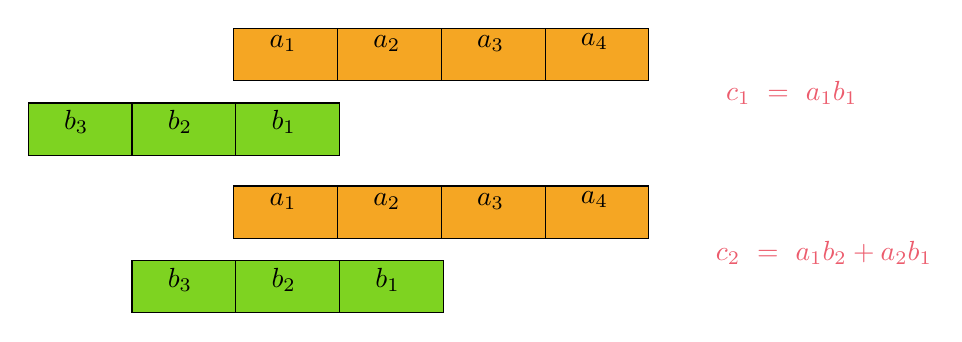
\begin{tikzpicture}[x=0.75pt,y=0.75pt,yscale=-1,xscale=1]
    %uncomment if require: \path (0,300); %set diagram left start at 0, and has height of 300
    
    %Shape: Rectangle [id:dp6383640467867335] 
    \draw  [fill={rgb, 255:red, 245; green, 166; blue, 35 }  ,fill opacity=1 ] (110,54) -- (160.01,54) -- (160.01,79.16) -- (110,79.16) -- cycle ;
    
    %Shape: Rectangle [id:dp9915913508162717] 
    \draw  [fill={rgb, 255:red, 245; green, 166; blue, 35 }  ,fill opacity=1 ] (260.01,54) -- (310.02,54) -- (310.02,79.16) -- (260.01,79.16) -- cycle ;
    %Shape: Rectangle [id:dp7574544776550791] 
    \draw  [fill={rgb, 255:red, 245; green, 166; blue, 35 }  ,fill opacity=1 ] (210,54) -- (260.01,54) -- (260.01,79.16) -- (210,79.16) -- cycle ;
    %Shape: Rectangle [id:dp15668905720803483] 
    \draw  [fill={rgb, 255:red, 245; green, 166; blue, 35 }  ,fill opacity=1 ] (160,54) -- (210.01,54) -- (210.01,79.16) -- (160,79.16) -- cycle ;
    
    %Shape: Rectangle [id:dp517800094810728] 
    \draw  [fill={rgb, 255:red, 126; green, 211; blue, 33 }  ,fill opacity=1 ] (11,90) -- (61.01,90) -- (61.01,115.16) -- (11,115.16) -- cycle ;
    %Shape: Rectangle [id:dp15583903887589012] 
    \draw  [fill={rgb, 255:red, 126; green, 211; blue, 33 }  ,fill opacity=1 ] (61,90) -- (111.01,90) -- (111.01,115.16) -- (61,115.16) -- cycle ;
    %Shape: Rectangle [id:dp4794201673076599] 
    \draw  [fill={rgb, 255:red, 126; green, 211; blue, 33 }  ,fill opacity=1 ] (111,90) -- (161.01,90) -- (161.01,115.16) -- (111,115.16) -- cycle ;
    
    %Shape: Rectangle [id:dp9652913856506695] 
    \draw  [fill={rgb, 255:red, 245; green, 166; blue, 35 }  ,fill opacity=1 ] (110,130) -- (160.01,130) -- (160.01,155.16) -- (110,155.16) -- cycle ;
    
    %Shape: Rectangle [id:dp6681556567962323] 
    \draw  [fill={rgb, 255:red, 245; green, 166; blue, 35 }  ,fill opacity=1 ] (260.01,130) -- (310.02,130) -- (310.02,155.16) -- (260.01,155.16) -- cycle ;
    %Shape: Rectangle [id:dp0819288495364412] 
    \draw  [fill={rgb, 255:red, 245; green, 166; blue, 35 }  ,fill opacity=1 ] (210,130) -- (260.01,130) -- (260.01,155.16) -- (210,155.16) -- cycle ;
    %Shape: Rectangle [id:dp015621153657017217] 
    \draw  [fill={rgb, 255:red, 245; green, 166; blue, 35 }  ,fill opacity=1 ] (160,130) -- (210.01,130) -- (210.01,155.16) -- (160,155.16) -- cycle ;
    
    %Shape: Rectangle [id:dp9772799588063847] 
    \draw  [fill={rgb, 255:red, 126; green, 211; blue, 33 }  ,fill opacity=1 ] (61,166) -- (111.01,166) -- (111.01,191.16) -- (61,191.16) -- cycle ;
    %Shape: Rectangle [id:dp8281584537494973] 
    \draw  [fill={rgb, 255:red, 126; green, 211; blue, 33 }  ,fill opacity=1 ] (111,166) -- (161.01,166) -- (161.01,191.16) -- (111,191.16) -- cycle ;
    %Shape: Rectangle [id:dp20253755057026024] 
    \draw  [fill={rgb, 255:red, 126; green, 211; blue, 33 }  ,fill opacity=1 ] (161,166) -- (211.01,166) -- (211.01,191.16) -- (161,191.16) -- cycle ;
    
    
    % Text Node
    \draw (126,56.4) node [anchor=north west][inner sep=0.75pt]    {$a_{1}$};
    % Text Node
    \draw (176,56.4) node [anchor=north west][inner sep=0.75pt]    {$a_{2}$};
    % Text Node
    \draw (226,56.4) node [anchor=north west][inner sep=0.75pt]    {$a_{3}$};
    % Text Node
    \draw (276,55.4) node [anchor=north west][inner sep=0.75pt]    {$a_{4}$};
    % Text Node
    \draw (127,92.4) node [anchor=north west][inner sep=0.75pt]    {$b_{1}$};
    % Text Node
    \draw (77,92.4) node [anchor=north west][inner sep=0.75pt]    {$b_{2}$};
    % Text Node
    \draw (27,92.4) node [anchor=north west][inner sep=0.75pt]    {$b_{3}$};
    % Text Node
    \draw (77,168.4) node [anchor=north west][inner sep=0.75pt]    {$b_{3}$};
    % Text Node
    \draw (127,168.4) node [anchor=north west][inner sep=0.75pt]    {$b_{2}$};
    % Text Node
    \draw (177,168.4) node [anchor=north west][inner sep=0.75pt]    {$b_{1}$};
    % Text Node
    \draw (276,131.4) node [anchor=north west][inner sep=0.75pt]    {$a_{4}$};
    % Text Node
    \draw (226,132.4) node [anchor=north west][inner sep=0.75pt]    {$a_{3}$};
    % Text Node
    \draw (176,132.4) node [anchor=north west][inner sep=0.75pt]    {$a_{2}$};
    % Text Node
    \draw (126,132.4) node [anchor=north west][inner sep=0.75pt]    {$a_{1}$};
    % Text Node
    \draw (346,78.4) node [anchor=north west][inner sep=0.75pt]  [color={rgb, 255:red, 236; green, 92; blue, 109 }  ,opacity=1 ]  {$c_{1} \ =\ a_{1} b_{1}$};
    % Text Node
    \draw (341,155.4) node [anchor=north west][inner sep=0.75pt]  [color={rgb, 255:red, 236; green, 92; blue, 109 }  ,opacity=1 ]  {$c_{2} \ =\ a_{1} b_{2} +a_{2} b_{1}$};
    
    
    \end{tikzpicture}
    
$$\begin{aligned}
    c_{1}&=a_{1} b_{1}\\
    c_{2}&=a_{1} b_{2}+a_{2} b_{1}\\
    c_{3}&=a_{1} b_{3}+a_{2} b_{2}+a_{3} b_{1}\\
    c_{4}&=a_{2} b_{3}+a_{3} b_{2}+a_{4} b_{1}\\
    c_{5}&=a_{3} b_{3}+a_{4} b_{2}\\
    c_{6}&=a_{4} b_{3}\\
\end{aligned} $$


\end{example}

\begin{corollary}
    假设向量$a$和$b$分别是以下多项式的系数
    $$ p(x)=a_{1}+a_{2} x+\cdots+a_{n} x^{n-1}, q(x)=b_{1}+b_{2} x+\cdots+b_{m} x^{m-1} $$

    则 $ \mathrm{c}=\mathrm{a}^{*} \mathrm{~b} $ 是多项式 $ p(x) q(x) $ 的系数.

    $$ p(x) q(x)=c_{1}+c_{2} x+\cdots+c_{m+n-1} x^{m+n-2} $$
\end{corollary}

\begin{corollary}[卷积性质]
    有如下性质:
    \begin{itemize}
        \item 对称性: $ a * b=b * a $
        \item 结合律: $ (a * b) * c=a *(b * c) $
        \item 如果 $ a * b=0 $, 则 $ a=0 $, 或者 $ b=0 $
    \end{itemize}
\end{corollary}

\begin{corollary}
    如果固定 $ a $或$b$,则 $ c=a * b $ 是一个线性函数
\end{corollary}

\begin{example}[Toeplitz Matrix]
    4维向量a和3维向量 $ b $ ,  则 $ c=a * b $

$$
\left[\begin{array}{l}
c_{1} \\
c_{2} \\
c_{3} \\
c_{4} \\
c_{5} \\
c_{6}
\end{array}\right]=\left[\begin{array}{lll}
a_{1} & 0 & 0 \\
a_{2} & a_{1} & 0 \\
a_{3} & a_{2} & a_{1} \\
a_{4} & a_{3} & a_{2} \\
0 & a_{4} & a_{3} \\
0 & 0 & a_{4}
\end{array}\right]\left[\begin{array}{l}
b_{1} \\
b_{2} \\
b_{3}
\end{array}\right]=\left[\begin{array}{cccc}
b_{1} & 0 & 0 & 0 \\
b_{2} & b_{1} & 0 & 0 \\
b_{3} & b_{2} & b_{1} & 0 \\
0 & b_{3} & b_{2} & b_{1} \\
0 & 0 & b_{3} & b_{2} \\
0 & 0 & 0 & b_{3}
\end{array}\right]\left[\begin{array}{l}
a_{1} \\
a_{2} \\
a_{3} \\
a_{4}
\end{array}\right]
$$
\end{example}

\subsection{多项式}

\begin{definition}[多项式]
    \textit{多项式} $ p(t) $, \textit{度}为 $ n-1 $, \textit{系数}为 $ x_{1}, x_{2}, \ldots, x_{n} $

    $$
p(t)=x_{1}+x_{2} t+x_{3} t^{2}+\cdots+x_{n} t^{n-1}
$$
\end{definition}

\begin{definition}[Vandermonde Matrices]
    $ \mathrm{p}(\mathrm{t}) $ 在m个点中 $ t_{1}, t_{2}, \ldots, t_{m} $ 的值为
    $$
    \left[\begin{array}{c}
    p\left(t_{1}\right) \\
    p\left(t_{2}\right) \\
    \vdots \\
    p\left(t_{m}\right)
    \end{array}\right]=\left[\begin{array}{cccc}
    1 & t_{1} & \cdots & t_{1}^{n-1} \\
    1 & t_{2} & \cdots & t_{2}{ }^{n-1} \\
    \vdots & \vdots & \ddots & \vdots \\
    1 & t_{m} & \cdots & t_{m}{ }^{n-1}
    \end{array}\right]\left[\begin{array}{c}
    x_{1} \\
    x_{2} \\
    \vdots \\
    x_{n}
    \end{array}\right]=A x
    $$

    矩阵$A$被称为\textit{Vandermonde矩阵}.
\end{definition}

\subsection{Fourier Transform}

\begin{definition}[Discrete Fourier Transform (DFT)]
    DFT将 $ n $ 维复向量 $ x $ 映射为 $ {n} $ 维复向量 $ y\left(\mathbb{C}^{n} \rightarrow \mathbb{C}^{n}\right) $

    $$ y_{k}=\sum_{\ell=1}^{n} x_{\ell} e^{-i \frac{2 \pi}{n}(k-1)(\ell-1)}, k=1, \cdots, n $$

    $$ \left[\begin{array}{c}y_{1} \\ y_{2} \\ y_{3} \\ \vdots \\ y_{n}\end{array}\right]=\left[\begin{array}{ccccc}1 & 1 & 1 & \cdots & 1 \\ 1 & \omega^{-1} & \omega^{-2} & \cdots & \omega^{-(n-1)} \\ 1 & \omega^{-2} & \omega^{-4} & \cdots & \omega^{-2(n-1)} \\ \vdots & \vdots & \vdots & \cdots & \vdots \\ 1 & \omega^{-(n-1)} & \omega^{-2(n-1)} & \cdots & \omega^{-(n-1)(n-1)}\end{array}\right]\left[\begin{array}{c}x_{1} \\ x_{2} \\ x_{3} \\ \vdots \\ x_{n}\end{array}\right] $$

   其中 $ \omega=e^{2 \pi i / n} $.
\end{definition}

DFT矩阵W的第 $ k $ 行第 $ l $ 列的元素为 $ W_{k l}=\omega^{-(k-1)(l-1)} $.

\begin{definition}[Discrete Inverse Fourier Transform]
    $$ x_{\ell}=\frac{1}{n} \sum_{k=1}^{n} y_{k} e^{i \frac{2 \pi}{n}(k-1)(\ell-1)}, \ell=1, \cdots, n $$
\end{definition}

\subsection{Semi-Definite Matrices}

\begin{definition}[半正定矩阵]
    对称矩阵 $ A \in \mathbb{R}^{n \times n} $ 称为\textit{半正定矩阵}, 满足以下条件

$$
x^{T} A x \geq 0 \quad \forall x \in \mathbb{R}^{n}
$$
\end{definition}

\begin{definition}[正定矩阵]
    对称矩阵 $ A \in \mathbb{R}^{n \times n} $ 称为正定矩阵, 满足以下条件
$$
x^{T} A x>0 \quad \forall x \neq 0
$$
\end{definition}

\begin{definition}[二次型]
    如果对称矩阵 $ A \in \mathbb{R}^{n \times n} $, 则 $ x^{T} A x $ 是二次型
\end{definition}

\begin{proof}
    $$ x^{T} A x=\sum_{i=1}^{n} \sum_{j=1}^{n} x_{i} A_{i j} x_{j}=\sum_{i=1}^{n} A_{i i} x_{i}^{2}+2 \sum_{i>j} A_{i j} x_{i} x_{j} $$
\end{proof}

\begin{example}
    $$ A=\left[\begin{array}{ll}9 & 6 \\ 6 & a\end{array}\right] $$

    $$ x^{T} A x=9 x_{1}^{2}+12 x_{1} x_{2}+a x_{2}^{2}=\left(3 x_{1}+2 x_{2}\right)^{2}+(a-4) x_{2}^{2} $$

    如果 $ a>4 $, 矩阵 $ A $ 为正定矩阵:
$$
x^{T} A x>0 \quad \forall x \neq 0
$$

如果 $ a=4 $, 矩阵 $ A $ 为半正定矩阵, 但不是正定矩阵:
$$
x^{T} A x \geq 0 \quad \forall x, \quad x^{T} A x=0 \quad \exists x=\left[\begin{array}{l}
2 \\
-3
\end{array}\right]
$$

如果 $ a<4 $, 矩阵 $ A $ 不是半正定矩阵:
$$
x^{T} A x<0 \quad \exists x=\left[\begin{array}{l}
2 \\
-3
\end{array}\right]
$$
\end{example}

\begin{corollary}
    正定矩阵 $ A $ 都是非奇异的.
\end{corollary}

\begin{proof}
    $$ A x=0 \quad \Rightarrow \quad x^{T} A x=0 \quad \Rightarrow \quad x=0 $$

    最后一步由正定性得到的.($
    x^{T} A x>0 \quad \forall x \neq 0
    $)

\end{proof}

\begin{theorem}[正定矩阵对角元素性质]
    正定矩阵 $ A $ 有正的对角元素.

    $$
A_{i i}=e_{i}^{T} A e_{i}>0
$$
\end{theorem}

\begin{theorem}[半正定矩阵对角元素性质]
    每个半正定矩阵 $ A $ 都有非负的对角元素.
$$
A_{i i}=e_{i}^{T} A e_{i} \geq 0
$$
\end{theorem}

\begin{definition}[Gram矩阵]
    Gram矩阵 $ A $

    $$ A=B^{T} B $$
\end{definition}

\begin{theorem}
    每个Gram矩阵都是半正定的.
\end{theorem}

\begin{proof}
    $$ x^{T} A x=x^{T} B^{T} B x=\|B x\|_{2}^{2} \geq 0 , \forall x $$
\end{proof}

\begin{theorem}
    如果Gram矩阵是正定的, 则要满足
    $$ x^{T} A x=x^{T} B^{T} B x=\|B x\|_{2}^{2}>0 ( \forall x \neq 0) $$
\end{theorem}

\begin{corollary}
    如果Gram矩阵是正定的, 则$B$的列向量是线性无关的.
\end{corollary}

\begin{proof}
    $$\|B x\|_{2}^{2}>0 ( \forall x \neq 0)$$

所以 $\forall x \neq 0, Bx \neq 0  $.

    注意和线性无关 \ref{Def:LinearIndependence} 的定义进行参照.
\end{proof}

\chapter{Matrices Norms}

\section{矩阵范数}

\begin{definition}[Matrix Norm]
    向量空间中存在一个函数 $ \|\cdot\|: \mathbb{R}^{m \times n} \rightarrow \mathbb{R} $

    且满足以下条件:

    \begin{itemize}
        \item 齐次性: $ \|\alpha A\|=|\alpha|\|A\|, \alpha \in \mathbb{R} $ 且 $ A \in \mathbb{R}^{m \times n} $;
        \item 三角不等式: $ \|A+B\| \leq\|A\|+\|B\|, A, B \in \mathbb{R}^{m \times n} $;
        \item 非负性: $ \|A\| \geq 0, A \in \mathbb{R}^{m \times n} $ 且 $ \|A\|=0 \Leftrightarrow A=0 $;
    \end{itemize}

则称 $ \|\cdot\| $ 为矩阵范数. 
\end{definition}

向量空间 $ \mathbb{R}^{m \times n} $ 矩阵范数:

\begin{example}[F-范数(Frobenius norm)]
    $$ \|A\|_{F}=\left(\sum_{i=1}^{n} \sum_{j=1}^{n} a_{i j}^{2}\right)^{\frac{1}{2}} $$
\end{example}

\begin{proof}
    $$ \|A\|_{F} \geq 0 $$

    $$ \|\alpha A\|_{F}=|\alpha|\|A\|_{F}, \alpha \in \mathbb{R} $$

    $$ \begin{aligned}\|A+B\|_{F}=&\left(\sum_{i=1}^{n} \sum_{j=1}^{n}\left(a_{i j}+b_{i j}\right)^{2}\right)^{\frac{1}{2}} \leq\left(\sum_{i=1}^{n} \sum_{j=1}^{n}\left(a_{i j}\right)^{2}\right)^{\frac{1}{2}}+\left(\sum_{i=1}^{n} \sum_{j=1}^{n}\left(b_{i j}\right)^{2}\right)^{\frac{1}{2}} \\ &=\|A\|_{F}+\|B\|_{F} \end{aligned} $$
\end{proof}

\begin{definition}[从属于给定向量范数 $ \|x\|_{v} $ 的矩阵范数]
    设 $ x \in \mathbb{R}^{n}, A \in \mathbb{R}^{m \times n},\|\cdot\|_{v} $ 为一种向量范数. 则 $ \frac{\|A x\|_{v}}{\|x\|_{v}} $ 对所有 $ x \neq 0 $ 有最大值, 令

    $$ \|A\|_{v}=\max _{x \neq 0}\left\{\frac{\|A x\|_{v}}{\|x\|_{v}}\right\}=\max _{x \neq 0}\left\{\left\|A \frac{x}{\|x\|_{v}}\right\|_{v}\right\}=\max _{\|y\|_{v}=1}\left\{\|A y\|_{v}\right\} $$

    即$$ \|A\|_{v}=\max _{x \neq 0}\left\{\frac{\|A x\|_{v}}{\|x\|_{v}}\right\} $$

    $ \|A\|_{v} $ 称为从属于给定向量范数 $ \|x\|_{v} $ 的矩阵范数, 简称为从属范数或算子范数.
\end{definition}

\begin{proof}
    可以验证 $ \|A\|_{v} $ 满足矩阵范数定义. 

    $$ \|A\|_{v} \geq 0 $$

    $$ \|\alpha A\|_{v}=|\alpha|\|A\|_{v}, \alpha \in \mathbb{R} $$

    $$\begin{aligned}
        \|A+B\|_{v} &=\max _{\|y\|_{v}=1}\|(A+B) y\|_{v} \\
        &\leq \max _{\|y\|_{v}=1}\left\{\|A y\|_{v}+\|B y\|_{v}\right\} \\
        & \leq \max _{\|y\|_{v}=1}\|A y\|_{v}+\max _{\|y\|_{v}=1}\|B y\|_{v} \\
        & =\|A\|_{v}+\|B\|_{v}
    \end{aligned}$$

\end{proof}

\begin{remark}
    在本书中若未明确说明, $\|A \|$表示的是算子范数.
\end{remark}

由定义 $ \|A\|_{v}=\max _{x \neq 0}\left\{\frac{\|A x\|_{v}}{\|x\|_{v}}\right\} $ 可得

\begin{definition}[向量范数和算子范数相容]
    $$ \frac{\|A x\|_{v}}{\|x\|_{v}} \leq\|A\|_{v} \Rightarrow\|A x\|_{v} \leq\|A\|_{v}\|x\|_{v} $$

    称向量范数和算子范数\textit{相容}. 
\end{definition}

\begin{theorem}[算子范数服从乘法范数相容性]
   对于 $ A \in \mathbb{R}^{m \times n}, B \in \mathbb{R}^{n \times p} $

    $$\begin{aligned}
        \|A B\|_{v} &=\max _{x \neq 0}\left\{\frac{\|A B x\|_{v}}{\|x\|_{v}}\right\} \\
        & \leq \max _{x \neq 0}\left\{\frac{\|A\|_{v}\|B x\|_{v}}{\|x\|_{v}}\right\} \\
        & \leq\|A\|_{v} \max _{x \neq 0}\left\{\frac{\|B\|_{v}\|x\|_{v}}{\|x\|_{v}}\right\} \\
        & =\|A\|_{v}\|B\|_{v}
    \end{aligned}$$
    算子范数服从\textit{乘法范数相容性}.
\end{theorem}

根据向量的常用范数可以导出矩阵 $ A \in \mathbb{R}^{m \times n} $ 的算子范数

\begin{definition}[$A$的列范数]
    $$ \|A\|_{1}=\max _{x \neq 0}\left(\frac{\|A x\|_{1}}{\|x\|_{1}}\right)=\max _{1 \leq j \leq n} \sum_{i=1}^{m}\left|a_{i j}\right| $$
\end{definition}

\begin{definition}[$A$的行范数]
    $$ \|A\|_{\infty}=\max _{x \neq 0}\left( \frac{\|A x\|_{\infty}}{\|x\|_{\infty}}    \right)=\max _{1 \leq i \leq m} \sum_{j=1}^{n}\left|a_{i j}\right| $$
\end{definition}

\begin{definition}[$A$的2−范数]
    $$ \|A\|_{2}=\max _{x \neq 0}\left( \frac{\|A x\|_{2}}{\|x\|_{2}}  \right)=\sqrt{\lambda_{\max }\left(A^{T} A\right)} $$
\end{definition}

\begin{example}
    求矩阵$A$的各种常用范数
$$
A=\left(\begin{array}{ccc}
1 & 2 & 0 \\
-1 & 2 & -1 \\
0 & 1 & 1
\end{array}\right)
$$

$$ \|A\|_{1}=\max _{1 \leq j \leq n} \sum_{i=1}^{n}\left|a_{i j}\right|=\max _{1 \leq j \leq n}\{2,5,2\}=5 $$

$$ \|A\|_{\infty}=\max _{1 \leq i \leq n} \sum_{j=1}^{n}\left|a_{i j}\right|=\max _{1 \leq i \leq n}\{3,4,2\}=4 $$

由于 $ \|A\|_{2}=\sqrt{\lambda_{\max }\left(A^{T} A\right)} $
, 因此先求 $ A^{T} A $ 的特征值

$$ A^{T} A=\left(\begin{array}{ccc}1 & -1 & 0 \\ 2 & 2 & 1 \\ 0 & -1 & 1\end{array}\right) \cdot\left(\begin{array}{ccc}1 & 2 & 0 \\ -1 & 2 & -1 \\ 0 & 1 & 1\end{array}\right)=\left(\begin{array}{ccc}2 & 0 & 1 \\ 0 & 9 & -1 \\ 1 & -1 & 2\end{array}\right) $$

特征方程为

$$ \operatorname{det}\left(\lambda I-A^{T} A\right)=\left|\begin{array}{ccc}\lambda-2 & 0 & -1 \\ 0 & \lambda-9 & 1 \\ -1 & 1 & \lambda-2\end{array}\right|=0 $$

可得 $ A^{T} A $ 的特征值

$$ \lambda_{1}=9.1428, \lambda_{2}=2.9211, \lambda_{3}=0.9361 $$

\end{example}

\begin{remark}
    对于$\|A\|_{2}$需要计算$\lambda_{\max }\left(A^{T} A\right)$, 直接根据特征方程计算特征值的算法复杂度太高.
\end{remark}

\chapter{适定问题}

\section{The Definition of Well-posed Problem}

In 1923, the French mathematician Hadamard introduced the notion of well-posed (适定)  problem:

\begin{itemize}
    \item A solution for the problem exists;
    \item The solution is unique;
    \item Perturbations in the data should cause small perturbations in the solution.
\end{itemize}

One of these conditions is not satisfied, the problem is said to be ill-posed (病态) and demands a special consideration.

\begin{example}
    假设 $ A $ 是非奇异矩阵 $$ A x=b $$

    如果将 $ b $ 为 $ b+\Delta b $, 方程新的解 $ x+\Delta x $, 则有:
$$
A(x+\Delta x)=b+\Delta b
$$

即
$$
\Delta x=A^{-1} \Delta b
$$

如果小的变化 $ \Delta b $ 导致小变化 $ \Delta x $, 则称解是\textit{稳定}的. 如果小的变化 $ \Delta b $ 导致大变化 $ \Delta x $, 则称解\textit{不稳定}的. 

设$$ A=\frac{1}{2}\left[\begin{array}{cc}1 & 1 \\ 1+10^{-10} & 1-10^{-10}\end{array}\right], \quad A^{-1}=\left[\begin{array}{cc}1-10^{10} & 10^{10} \\ 1+10^{10} & -10^{10}\end{array}\right] $$

若$ b=(1,1) $, 方程 $ A x $ 的解 $ x=(1,1) $ . 
如果将b改为 $ b+\Delta b $ , 那么 $ x $ 的变化量为

$$ \Delta x=A^{-1} \Delta b=\left[\begin{array}{l}\Delta b_{1}-10^{10}\left(\Delta b_{1}-\Delta b_{2}\right) \\ \Delta b_{1}+10^{10}\left(\Delta b_{1}-\Delta b_{2}\right)\end{array}\right] $$

很小变化 $ \Delta b $ 会导致非常大变化 $ \Delta x $! 由矩阵$A$定义的问题, 称为\textit{适定问题}或\textit{病态问题}. 

\end{example}

\section{绝对误差的界限}

假设 $ A $ 是非奇异的, 并给出定义:

\begin{notation}
    $$ x=A^{-1} b$$ 
    
    $$ \Delta x=A^{-1} \Delta b $$
\end{notation}

$ \|\Delta x\| $ 的上界为:
$$
\|\Delta x\|_{2} \leq\left\|A^{-1}\right\|_{2}\|\Delta b\|_{2}
$$

矩阵范数 $ \left\|A^{-1}\right\|_{2} $ 小时, 当 $ \|\Delta b\|_{2} $ 变化很小, $ \|\Delta x\|_{2} $ 也很小; $ \left\|A^{-1}\right\|_{2} $ 大时,  $ \|\Delta x\|_{2} $ 可能很大,  即使 $ \|\Delta b\|_{2} $ 很小. 

\section{相对误差的界限}

假设 $ b \neq 0 $; 因此 $ x \neq 0$

$\|\Delta x\|_{2} /\|x\|_{2} $ 的上界为:

$$ 
\begin{aligned}
    &\|\Delta x\|_{2}=\left\|A^{-1} \Delta b\right\|_{2} \leq\left\|A^{-1}\right\|_{2}\|\Delta b\|_{2}(向量范数和算子范数相容)\\
    \Rightarrow& \frac{\|\Delta x\|_{2}}{\|x\|_{2}} \leq \frac{\left\|A^{-1}\right\|_{2}\|\Delta b\|_{2}}{\|x\|_{2}}=\frac{\|A\|_{2}\left\|A^{-1}\right\|_{2}\|\Delta b\|_{2}}{\|x\|_{2}\|A\|_{2}} \leq \frac{\|A\|_{2}\left\|A^{-1}\right\|_{2}\|\Delta b\|_{2}}{\|b\|_{2}}
\end{aligned}
$$

由 $ \|b\|_{2}=\|A x\|_{2} \leq\|A\|_{2}\|x\|_{2} $, 可得

$$ \frac{\|\Delta x\|_{2}}{\|x\|_{2}} \leq\|A\|_{2}\left\|A^{-1}\right\|_{2} \frac{\|\Delta b\|_{2}}{\|b\|_{2}} $$

$ \|A\|_{2}\left\|A^{-1}\right\|_{2} $ 小,当 $ \|\Delta b\|_{2} /\|b\|_{2} $ 相对变化很小时, $ \|\Delta x\|_{2} /\|x\|_{2} $ 也 变化很小;

$ \|A\|_{2}\left\|A^{-1}\right\|_{2} $ 大, $ \|\Delta x\|_{2} /\|x\|_{2} $ 可远远大于 $ \|\Delta b\|_{2} /\|b\|_{2} $.


\begin{definition}[非奇异矩阵 $ A $ 的条件数(condition number)]
    $$ \kappa(A)=\|A\|_{2}\left\|A^{-1}\right\|_{2} $$
\end{definition}

\begin{corollary}[非奇异矩阵 $ A $ 的条件数(condition number)性质]
    有如下性质:

    \begin{itemize}
        \item 对于所有 $ A $, 有 $ \kappa(A) \geq 1 $;
        \item 如果 $ \kappa(A) $ 比较小 (接近1),  $ x $ 的相对误差接近 $ b $ 的相对误差;
        \item 如果 $ \kappa(A) $ 比较大(超过100),  $ x $ 的相对误差比 $ b $ 的相对误差大得多. 
    \end{itemize}
\end{corollary}


